\scanpage{72}
\mspage{71}
% E: text|upper left|Je voudrais revenir à la question
Je voudrais revenir à la question de faire une surface avec les p.r. \uline{stables}. Pour une telle $D$, $\Delta_D$ n'a comme arcs de transition que des arcs de \uline{spécialisation}. Comment raccorder $\Delta_D$ et $\Delta_{D'}$, quand $D,D'$ sont déduits l'une de l'autre par balayage au dessus d'un sommet?
% E: drawing|left middle|D and D' passing on opposite sides of s
\figure{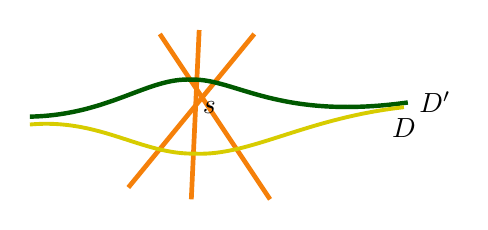
\begin{tikzpicture}[x=1cm,y=1cm]
\draw[orange!85!brown,line width=1.7pt] (-.85,1.05)--(.55,-1.05);
\draw[orange!85!brown,line width=1.7pt] (-.35,1.1)--(-.45,-1.05);
\draw[orange!85!brown,line width=1.7pt] (.35,1.05)--(-1.25,-.9);
\draw[green!35!black,line width=1.6pt] (-2.5,0) .. controls (-1.5,.02) and (-1,.5) .. (-.45,.47) .. controls (.1,.49) and (.65,-.05) .. (2.3,.18) node[right,black] {$D'$};
\draw[yellow!65!olive,line width=1.4pt] (-2.5,-.1) .. controls (-1.6,-.02) and (-1.1,-.48) .. (-.4,-.47) .. controls (.3,-.5) and (1,-.02) .. (2.25,.12) node[below,black] {$D$};
\node at (-.22,.12) {$\unsure{s}$};
\end{tikzpicture}}
% E: text|left middle beside figure continuing below|Ici il n'y a pas d'ambiguïté
Ici, il n'y a pas d'ambiguïté possible sur les arcs le long desquels faire le recollement, \unsure{ni} \unsure{par|sur} l'interprétation des \unsure{arcs de spécialisation non plus} (il faudrait du vice pour \unsure{l'antipodisme} pour recoller!). Ici, il est très tentant de remplacer encore $\Delta_D,\Delta_{D'}$ par $\Delta_D^*,\Delta_{D'}^*$ déduits en balayant les bords jusqu'au point $s$ ``critique'' qui nous intéresse, \deleted{\unsure{pour}} de recoller.
% E: margin note|left margin at il faudrait du vice|exclamation and vertical emphasis
\margin{!\ \figure{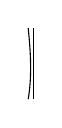
\begin{tikzpicture}[baseline]\draw (0,0)..controls(.05,.3)and(.03,.6)..(0,.9);\draw(.07,0)--(.07,.9);\end{tikzpicture}}}
% E: insertion|left lower middle above à partir|Revenant aux figures symétriques
\inserted{\unsure{Revenant} aux figures symétriques}
% E: text|bottom left continuing right|à partir de la position semi-stable
(à partir de la position semi-stable intermédiaire) on a à priori $8$ possibilités de recollement, suivant \deleted{les \unsure{quatre}} quatre choix d'\unsure{éléments} dans $\{a,a'\}\times\{b,b'\}$, puis le choix d'orientation pour recoller $\alpha\in\{a,a'\}$ avec $\beta\in\{b,b'\}$. Mais déjà le choix d'un couple $(a,b')$ ou $(b,a')$ est exclu, à cause de la nécessaire symétrie temporelle. Donc il reste deux couples $(a,b),(a',b')$, et pour chacun choix parmi les deux possibilités de recollage --- transport parallèle, ou l'opposé. Mais modulo \deleted{\unsure{application}} transformation, par antipodismes de part et d'autre (qui ne \unsure{change pas} la surface $\mathcal X$ \unsure{obtenue par recollement} \unsure{sans $D$ car disparu de la donnée|sans $D$ car disponible en la donnée}) \unsure{cas|des} $(a,b)$.
% E: drawing|top right cancelled pair|a a' and adjacent pencil outline
\deleted{\figure{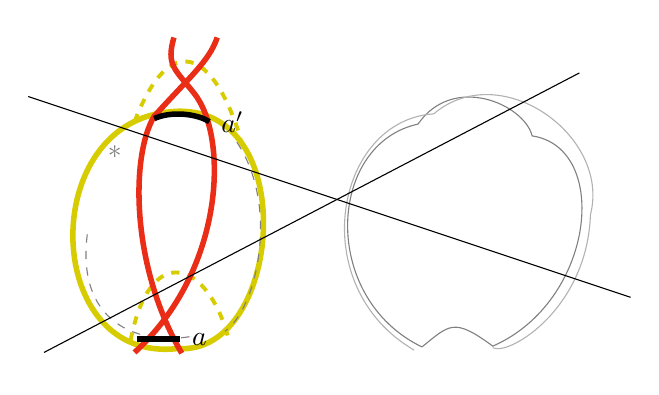
\begin{tikzpicture}[x=1cm,y=1cm]
\draw[yellow!65!olive,line width=2pt] (0,0) .. controls (-1.7,-.2) and (-1.8,2.8) .. (-.15,3) .. controls (1.6,3.25) and (1.35,-.1) .. (0,0);
\draw[yellow!65!olive,dashed,line width=1.4pt] (-.55,2.88)..controls(-.1,4.05)and(.45,3.8)..(.8,2.66);
\draw[yellow!65!olive,dashed,line width=1.4pt] (-.6,.1)..controls(-.35,1.4)and(.4,1.1)..(.65,.1);
\draw[gray,dashed] (-1.15,1.45)..controls(-1.3,.25)and(-.4,.02)..(.25,.17);
\draw[gray,dashed] (.75,2.62)..controls(1.3,1.8)and(1,.5)..(.6,.22);
\draw[red!65!brown,line width=2pt] (-.55,-.05)..controls(.6,1)and(.65,2.7)..(.2,3.25)..controls(-.04,3.55)and(-.15,3.6)..(-.05,3.95);
\draw[red!65!brown,line width=2pt] (.05,-.06)..controls(-.6,1.05)and(-.6,2.45)..(-.3,2.95)..controls(.15,3.45)and(.4,3.65)..(.5,3.95);
\draw[line width=2pt] (-.3,2.92)..controls(-.08,3.02)and(.25,2.98)..(.4,2.88) node[right] {$a'$};
\draw[line width=2pt] (-.52,.12)--(.03,.12) node[right] {$a$};
\node[gray] at (-.8,2.5) {$\unsure{*}$};
\draw[gray] (3.1,.02)..controls(1.8,.65)and(1.9,2.6)..(3.05,2.85)..controls(3.5,3.5)and(4.4,3.1)..(4.5,2.7)..controls(5.5,2.55)and(5.3,.6)..(4,.03)..controls(3.5,.4)and(3.45,.3)..(3.1,.02);
\draw[gray!60] (3,-.02)..controls(1.6,.8)and(2,2.9)..(3.25,2.98)..controls(4.1,3.7)and(5.5,2.7)..(5.24,1.7)..controls(5.2,.5)and(4.2,-.1)..(4,.01);
\draw (-1.9,3.2)--(5.75,.65);\draw(-1.7,-.05)--(5.1,3.5);
\end{tikzpicture}}}
% E: drawing|right middle|four arcs a a' b b'
\figure{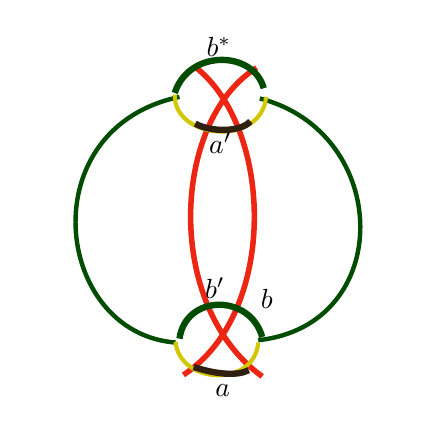
\begin{tikzpicture}[x=1cm,y=1cm]
\draw[green!30!black,line width=1.6pt] (-.5,3.25)..controls(-2.4,2.85)and(-2.1,.25)..(-.55,.13);
\draw[green!30!black,line width=1.6pt] (.52,3.23)..controls(2.2,2.8)and(2.25,.35)..(.5,.16);
\draw[red!70!brown,line width=2pt] (-.45,-.28)..controls(.75,.5)and(.7,2.85)..(-.3,3.63);
\draw[red!70!brown,line width=2pt] (.55,-.3)..controls(-.7,.6)and(-.6,2.95)..(.48,3.62);
\draw[yellow!60!olive,line width=1.5pt] (-.56,3.28)..controls(-.58,2.71)and(.54,2.61)..(.6,3.25);
\draw[green!30!black,line width=2.3pt] (-.56,3.3)..controls(-.38,3.86)and(.44,3.84)..(.57,3.36);
\draw[black!75!brown,line width=2.3pt] (-.3,2.91)..controls(-.1,2.8)and(.28,2.8)..(.4,2.94);
\draw[yellow!60!olive,line width=1.5pt] (-.55,.14)..controls(-.5,-.4)and(.45,-.45)..(.5,.13);
\draw[green!30!black,line width=2.3pt] (-.5,.18)..controls(-.42,.75)and(.4,.75)..(.55,.2);
\draw[black!75!brown,line width=2.3pt] (-.32,-.18)..controls(-.05,-.27)and(.23,-.3)..(.38,-.22);
\node at (0,3.89) {$b^{\deleted{\unsure{*}}}$};
\node at (.02,2.66) {$a'$};\node at (-.05,.82) {$b'$};
\node at (.61,.69) {$\deleted{\unsure{b}}$};\node at (.05,-.48) {$a$};
\end{tikzpicture}}
